The symbolic and embedding-based approaches discussed so far purely rely on a knowledge graph's facts for prediction. This section presents models that leverage additional information, such as type information, textual entity descriptions, or logical rules to improve their predictions.

Type information is provided by some knowledge graphs to distinguish between different kinds of entities. A graph representing a social network, for example, might label entities as persons, locations, or events. A simple model that leverages such type information is SSE~\cite{Guo2015SemanticallySK}, which keeps entities of the same type closer together during training. One of its drawbacks, however, is that it can only handle non-hierarchical types. In contrast TKRL~\cite{Xie2016RepresentationLO} extends on this and supports hierarchical types as well as multiple type labels per entity. Another advantage of typed knowledge graphs is that types can be used to improve negative sampling: By excluding augmented negative samples with correct typings it can be guaranteed that no true facts are generated.

Another kind of additional information, and arguably the most comprehensive one, is textual entity descriptions. Dictionaries and encyclopedias contain concise definitions and descriptions for a wide range of entities and web crawlers can collect texts from vast online sources. The NTN~\cite{Socher2013ReasoningWN} model mentioned before was one of the first KGC models to leverage that information to initialize its entity embeddings by averaging the word embeddings of the entities' names. Similarly Long et al. used longer text descriptions to initialize entity embeddings~\cite{Long2016LeveragingLR}. However, both approaches have in common that the texts are not used to improve fact embeddings during training.

One of the earliest approaches to use texts beyond entity initialization was proposed by Wang et al.~\cite{Wang2014KnowledgeGE} who implemented joint embedding of facts and texts. Later, DKRL~\cite{Xie2016RepresentationLO}, an extension to TransE, and OWE~\cite{Shah2019AnOE}, an extension to embedding-based KGC models in general, have been developed. Both have the advantage that they can also be applied to open-world entities that are not seen during training. \autoref{fig:3_related_work/3_additional_information/owe} illustrates the working of OWE: First, word embedding and graph embedding models are trained separately on the text and graph data. Then, an alignment function $\psi$ is learned that maps word embeddings to their respective entity embeddings. This allows texts of open-world entities to be mapped to the right position in the graph embedding space. In the example in \autoref{fig:3_related_work/3_additional_information/owe}, it would thus be possible to predict similar facts for the open-world entity John as for the known entity Ed it is close to.

\begin{figure}[t]
    \centering
    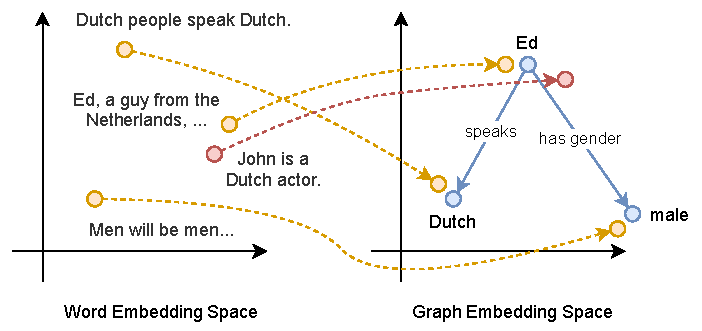
\includegraphics{3_related_work/3_additional_information/owe}
    \caption{The OWE model~\cite{Shah2019AnOE} learns a mapping function to align its separately learned word and graph embedding spaces, which allows predictions for open-world entities. Here, the text of the open-world entity John (red) is embedded close to the text of the known entity Ed, leading to similar embeddings in the graph embedding space, allowing OWE to predict similar facts for John.}
    \label{fig:3_related_work/3_additional_information/owe}
\end{figure}

Finally, beyond type and text information, some models also attempted to incorporate rules into training of embedding-based models. Some early approaches~\cite{Wang2015KnowledgeBC, Wei2015LargescaleKB} used them to put constraints on their predicted facts, but such a post-processing step does not help with training the actual graph embedding. The KALE model~\cite{Guo2016JointlyEK} on the other hand represents facts and rules in a common vector space. The basic idea is to ground the rules and calculate the rule groundings' embeddings from the facts they consist of using fuzzy logics. The probability of a fact $(\textbf{h}, \textbf{r}, \textbf{t})$ is thereby based on the Manhatten distance between the $d$-dimensional vectors $\textbf{h} + \textbf{r}$ and $\textbf{t}$ as per Equation~\cite{eq:3_related_work/3_additional_information/kale_fact}, while \autoref{eq:3_related_work/3_additional_information/kale_rule} gives an example of how the probability of a rule grounding with two body facts $f_1$ and $f_2$ and a head fact $f_3$ is calculated.

\begin{align}
    I(\textbf{h}, \textbf{r}, \textbf{t}) &= 1 - \frac{1}{3 \sqrt {d}} {|| \textbf{h} + \textbf{r} - \textbf{t} ||}_1
    \label{eq:3_related_work/3_additional_information/kale_fact} \\
    I(f_1 \land f_2 \Rightarrow f_3) &= I(f_1) \cdot I(f_2) \cdot I(f_3) - I(f_1) \cdot I(f_2) + 1
    \label{eq:3_related_work/3_additional_information/kale_rule}
\end{align}

Beyond Horn rules, KALE can handle any propositional logic rules. Given the formula for calculating an arbitrary rule's probability, which includes single facts, KALE then employs a margin-based ranking loss to learn the common embedding space that allows looking up ground path rules that are similar to facts and vice versa. The only drawback is that KALE cannot handle quantifiers from first order logic, which is why it uses rule groundings.
